\subsection{Euclidean Cells and Cell Outer Measure}
\begin{definition} \label{def:measure-cells-intervals-volume-rp} \hlt{Cells, Intervals, and Volume in $\R^p$}
\begin{enumerate}[label=(\roman*)]
\setlength{\itemsep}{0pt}
\item \hlt{Cells in $\R$}. For $a\leq b$, a cell with endpoints $a,b$ is $I\in\{(a,b),[a,b],(a,b],[a,b)\}$, respectively open, closed, right-half-open, left-half-open; if $a=b$, only $[a,a]$ is nonempty.
\item \hlt{Length}. For a cell $I$ with endpoints $a\leq b$, $\ell(I)\defeq b-a$, independent of endpoint inclusion; $(-\infty,a)$, $(-\infty,a]$, $[b,+\infty)$, $(b,+\infty)$, and $\R$ are intervals, not cells, with length $+\infty$.
\item \hlt{Cells in $\R^p$}. For $p\geq1$, a cell is $I=\prod_{i=1}^{p}I_i$, each $I_i$ a cell in $\R$; its type is open, closed, or half-open, $\prod_i[a_i,b_i)$ is \hlt{southwest}, $\prod_i(a_i,b_i]$ is \hlt{northeast}, and a \hlt{cube} satisfies $\ell(I_1)=\cdots=\ell(I_p)$.
\item \hlt{Volume}. For $I=\prod_{i=1}^{p}I_i$, $\operatorname{vol}_p(I)\defeq\prod_{i=1}^{p}\ell(I_i)$ and $\operatorname{vol}_p(\emptyset)\defeq0$.\\
If endpoints are $a_i\leq b_i$, then $\operatorname{vol}_p(I)=\prod_{i=1}^{p}(b_i-a_i)$.
\item \hlt{Unbounded products}. For cells $I$, $\operatorname{vol}_p(I^\circ)=\operatorname{vol}_p(\overline I)=\operatorname{vol}_p(I)$.\\
For products $I=\prod_iI_i$ of possibly unbounded intervals, $\exists j:\ell(I_j)=0$ gives volume $0$, while $\ell(I_j)>0$ for all $j$ and $\exists j:\ell(I_j)=+\infty$ gives volume $+\infty$.
\end{enumerate}
\end{definition}

\begin{remark} \label{rem:cell-interval-topological-conventions} \hlt{Cells versus Intervals}\\
Cells are precisely bounded intervals with finite endpoints, so every cell is an interval but not conversely. Open cells are open in $\R^p$, closed cells are closed in $\R^p$, and nonempty half-open cells are neither.\\
In $\R$, $(-\infty,a)$ and $(b,+\infty)$ are open, $(-\infty,a]$ and $[b,+\infty)$ are closed, and $\R=(-\infty,+\infty)$ is clopen.\\
\hlt{Key Insight}: Topology likes open and closed endpoints; measure bookkeeping often likes half-open endpoints.
\end{remark}

\begin{proposition} \label{prop:half-open-cell-calculus-and-subdivision} \hlt{Half-Open Cell Calculus}\\
Fix $\sigma\in\{\hlt{southwest},\hlt{northeast}\}$, and let $\mathcal{H}_\sigma$ be the half-open cells in $\R^p$ with orientation $\sigma$.
\begin{enumerate}[label=(\roman*)]
\setlength{\itemsep}{0pt}
\item Any finite Boolean combination of $H_1,\ldots,H_n\in\mathcal{H}_\sigma$ is $\bigsqcup_{r=1}^{N}K_r$ with $K_r\in\mathcal{H}_\sigma$.
\item If $H\in\mathcal{H}_\sigma$, then $\R^p\setminus H=\bigsqcup_{r=1}^{\infty}K_r$ for some $K_r\in\mathcal{H}_\sigma$.
\item For $H\in\mathcal{H}_\sigma$ and $\delta>0$, $H=\bigsqcup_{r=1}^{N}K_r$ for some $K_r\in\mathcal{H}_\sigma$ with $\operatorname{diam}K_r<\delta$.
\end{enumerate}
\begin{proof}
\begin{enumerate}[label=(\roman*)]
\setlength{\itemsep}{0pt}
\item For coordinate endpoints $E_j=\{c_{j,0}<\cdots<c_{j,m_j}\}$ of $H_1,\ldots,H_n$, set $[a,b)_\sigma=[a,b)$ if $\sigma=\hlt{southwest}$ and $[a,b)_\sigma=(a,b]$ if $\sigma=\hlt{northeast}$, $\mathcal{P}_j=\{[c_{j,q-1},c_{j,q})_\sigma:1\leq q\leq m_j\}$, and $\mathcal{G}=\{\prod_{j=1}^{p}P_j:P_j\in\mathcal{P}_j\}$; every finite Boolean combination is $\bigsqcup_{G\in\mathcal{G}'}G$, $\mathcal{G}'\subseteq\mathcal{G}$.
\item Write $H=\prod_{j=1}^{p}H_j$ and $D_s=(\prod_{j<s}H_j)\times(\R\setminus H_s)\times\R^{p-s}$; then $\R^p\setminus H=\bigsqcup_{s=1}^{p}D_s$. Decomposing each one-dimensional ray and $\R$ into countably many bounded $\sigma$-half-open intervals and taking products gives the required union; countability follows from Corollary \ref{cor:countable-cartesian-products}.
\item Choose $m$ with $2^{-m}(\sum_{j=1}^{p}\ell(H_j)^2)^{1/2}<\delta$. After $m$ bisections per coordinate, each subcell has\\
diameter $<\delta$; disjointness and volume preservation follow coordinatewise.
\end{enumerate}
\hlt{Structural Commentary}: Half-open cells behave like grid atoms: finite set operations become finite grid selection.\\
\hlt{Key Insight}: Half-open endpoints prevent overlap while still partitioning boxes cleanly.
\end{proof}
\end{proposition}

\begin{definition} \label{def:translation-of-euclidean-set} \hlt{Translation of a Set}\\
If $A\subseteq\R^p$ and $t\in\R^p$, the translate of $A$ by $t$ is $t+A\defeq\{t+a:a\in A\}$.
\end{definition}

\begin{proposition} \label{prop:cell-volume-translation-invariant} \hlt{Cell Volume Is Translation Invariant}\\
Let $I=\prod_{i=1}^{p}I_i$ be a cell in $\R^p$ and $t=(t_i)_{i=1}^{p}\in\R^p$. Then $t+I=\prod_{i=1}^{p}(t_i+I_i)$ is a cell with the same endpoint pattern as $I$, and $\operatorname{vol}_p(t+I)=\operatorname{vol}_p(I)$.
\begin{proof}
Let $a_i\leq b_i$ be the endpoints of $I_i$. Then $t_i+I_i$ has endpoints $t_i+a_i\leq t_i+b_i$, unchanged endpoint inclusion, and $\ell(t_i+I_i)=(t_i+b_i)-(t_i+a_i)=\ell(I_i)$. Hence $\operatorname{vol}_p(t+I)=\prod_{i=1}^{p}\ell(t_i+I_i)=\prod_{i=1}^{p}\ell(I_i)=\operatorname{vol}_p(I)$.\\
\hlt{Structural Commentary}: Translation moves location but not side lengths.\\
\hlt{Key Insight}: Coordinate volume depends only on side lengths.
\end{proof}
\end{proposition}

\begin{definition} \label{def:elementary-sets-and-regular-set-functions} \hlt{Elementary Sets and Regularity in $\R^p$}
\begin{enumerate}[label=(\roman*)]
\setlength{\itemsep}{0pt}
\item \hlt{Elementary sets}. $\mathcal{E}\defeq\{\bigcup_{r=1}^{n}I_r:n\in\N\}$, where each $I_r\subseteq\R^p$ is a bounded cell.
\item \hlt{Elementary volume}. If $A=\bigsqcup_{r=1}^{n}I_r$ with cells $I_r$, set $m(A)\defeq\sum_{r=1}^{n}\operatorname{vol}_p(I_r)$.
\item \hlt{Regularity}. A nonnegative additive $\mu:\mathcal{E}\to[0,+\infty]$ is regular iff $\forall A\in\mathcal{E}$, $\forall\varepsilon>0$,\\
$\exists F,G\in\mathcal{E}$ with $F\subseteq A\subseteq G$, $F$ closed, $G$ open, and $\mu(G)-\varepsilon\leq\mu(A)\leq\mu(F)+\varepsilon$.
\end{enumerate}
$\mathcal{E}$ is a ring; every $A\in\mathcal{E}$ admits a finite disjoint cell decomposition; $m$ is well defined, additive, and regular.
\end{definition}

\begin{perspective} \label{per:box-volume-and-linear-algebra} \hlt{Box Volume and Linear Algebra}\\
For a box $B=\prod_i(a_i,b_i)$ or $\prod_i[a_i,b_i]$, $m(B)=\prod_i(b_i-a_i)$, the diagonal case of determinant volume scaling.\\
Measure extends this product rule beyond boxes.\\
\hlt{Key Insight}: Lebesgue measure starts from determinant-style coordinate volume.
\end{perspective}

\begin{perspective} \label{per:outer-measure-overestimation} \hlt{Outer Measure as Overestimation}\\
Elementary $A=\bigsqcup_{r=1}^{n}I_r$ have $m(A)=\sum_{r=1}^{n}\operatorname{vol}_p(I_r)$.\\
General $E\subseteq\R^p$, e.g. $D=\{(x,y)\in\R^2:x^2+y^2\leq1\}$, need not be a finite disjoint cell union.\\
Replace decompositions by countable cell covers $E\subseteq\bigcup_{k=1}^{\infty}I_k$ and minimize $\sum_{k=1}^{\infty}\operatorname{vol}_p(I_k)$.\\
\hlt{Key Insight}: Outer covers size every $E\subseteq\R^p$ before measurability.
\end{perspective}

\begin{definition} \label{def:cell-cover-outer-measure} \hlt{Cell-Cover Outer Measure}\\
For $E\subseteq\R^p$, let $\mathcal{C}(E)$ be the countable cell covers $(I_k)_{k\geq1}$ with $E\subseteq\bigcup\limits_{k=1}^{\infty}I_k$. Define $m_p^\ast(E)\defeq\inf\limits_{(I_k)\in\mathcal{C}(E)}\sum\limits_{k=1}^{\infty}\operatorname{vol}_p(I_k)$.
Here $\mathcal{C}(E)\neq\emptyset$ since $E\subseteq\bigcup\limits_{j=1}^{\infty}[-j,j]^p$, and sum is nonnegative extended-real series, hence order-independent.
\end{definition}

\begin{proposition} \label{prop:outer-measure-cover-normalizations} \hlt{Equivalent Covering Families}\\
For $E\subseteq\R^p$, $\delta>0$, and fixed half-open orientation $\sigma$, let $\mathcal{C}_{\mathsf{cl}}(E)$, $\mathcal{C}_{\mathsf{op}}(E)$, $\mathcal{C}_{\sigma}(E)$, and $\mathcal{C}_{\delta}(E)$ be the subfamilies of $\mathcal{C}(E)$ with cells respectively closed, open, $\sigma$-half-open, and satisfying $\operatorname{diam}I_k<\delta$.\\
If $\alpha(\mathcal{A})\defeq\inf_{(I_k)\in\mathcal{A}}\sum_{k=1}^{\infty}\operatorname{vol}_p(I_k)$, then $m_p^\ast(E)=\alpha(\mathcal{C}_{\mathsf{cl}}(E))=\alpha(\mathcal{C}_{\mathsf{op}}(E))=\alpha(\mathcal{C}_{\sigma}(E))=\alpha(\mathcal{C}_{\delta}(E))$.
\begin{proof}
Let $\mathcal{C}_\ast(E)$ be any restricted class above. Since $\mathcal{C}_\ast(E)\subseteq\mathcal{C}(E)$, $\alpha(\mathcal{C}_\ast(E))\geq m_p^\ast(E)$.\\
Conversely, for $(I_k)\in\mathcal{C}(E)$ and $\varepsilon>0$, closures give $\overline{I_k}\supseteq I_k$ and $\operatorname{vol}_p(\overline{I_k})=\operatorname{vol}_p(I_k)$; open cells $J_k\supseteq I_k$ may be chosen with $\operatorname{vol}_p(J_k)\leq\operatorname{vol}_p(I_k)+\varepsilon2^{-k}$; each $J_k$ admits a countable disjoint $\sigma$-half-open decomposition with total volume $\operatorname{vol}_p(J_k)$; each half-open cell has a finite disjoint subdivision into cells of diameter $<\delta$ with unchanged total volume. Thus $\alpha(\mathcal{C}_\ast(E))\leq\sum_k\operatorname{vol}_p(I_k)+\varepsilon$; take infima over $(I_k)$ and let $\varepsilon\downarrow0$.\\
\hlt{Structural Commentary}: Near-optimal covers ignore endpoint convention.\\
\hlt{Key Insight}: Closures, small enlargements, and fine subdivisions preserve the infimum.
\end{proof}
\end{proposition}

\begin{theorem} \label{thm:cell-cover-outer-measure-basic-properties} \hlt{Basic Properties of Cell-Cover Outer Measure}\\
For $E,F,E_n\subseteq\R^p$,
\begin{enumerate}[label=(\roman*)]
\setlength{\itemsep}{0pt}
\item \hlt{Null empty set}. $0\leq m_p^\ast(E)\leq+\infty$ and $m_p^\ast(\emptyset)=0$.
\item \hlt{Monotonicity}. $E\subseteq F\Longrightarrow m_p^\ast(E)\leq m_p^\ast(F)$.
\item \hlt{Subadditivity}. $m_p^\ast(\bigcup_{n=1}^{\infty}E_n)\leq\sum_{n=1}^{\infty}m_p^\ast(E_n)$.
\end{enumerate}
\begin{proof}
\begin{enumerate}[label=(\roman*)]
\setlength{\itemsep}{0pt}
\item Since all cover sums lie in $[0,+\infty]$, $0\leq m_p^\ast(E)\leq+\infty$; the cover $(\emptyset,\emptyset,\ldots)$ gives $m_p^\ast(\emptyset)=0$.
\item If $E\subseteq F$, then $\mathcal{C}(F)\subseteq\mathcal{C}(E)$, hence $\inf_{\mathcal{C}(E)}\leq\inf_{\mathcal{C}(F)}$.
\item If some $m_p^\ast(E_n)=+\infty$, the claim is trivial.\\
Otherwise, for $\varepsilon>0$, choose $(I_k^n)_{k\geq1}\in\mathcal{C}(E_n)$ with $\sum_k\operatorname{vol}_p(I_k^n)\leq m_p^\ast(E_n)+\varepsilon2^{-n}$.\\
Then $(I_k^n)_{(n,k)\in\N^2}$ countable, covers $\bigcup_nE_n$, and $m_p^\ast(\bigcup_nE_n)\leq\sum_{n,k}\operatorname{vol}_p(I_k^n)\leq\sum_nm_p^\ast(E_n)+\varepsilon$.
\end{enumerate}
\hlt{Structural Commentary}: Countable subadditivity is proved by merging near-optimal covers.\\
\hlt{Key Insight}: Nonnegative double sums may be scanned in one sequence.
\end{proof}
\end{theorem}

\begin{figure}[H]
  \centering
  % Source: The Elements of Lebesgue Measure, Ch. 12, Theorem 12.4 proof idea.
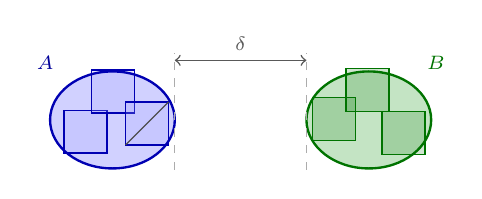
\begin{tikzpicture}[
  scale=0.88,
  every node/.style={font=\scriptsize},
  setAfill/.style={fill=blue!65, fill opacity=0.28, draw=none},
  setBfill/.style={fill=green!55!black, fill opacity=0.23, draw=none},
  setAline/.style={draw=blue!70!black, line width=0.85pt},
  setBline/.style={draw=green!45!black, line width=0.85pt},
  cellA/.style={fill=blue!35, fill opacity=0.22, draw=blue!70!black, line width=0.5pt},
  cellB/.style={fill=green!45!black, fill opacity=0.18, draw=green!45!black, line width=0.5pt},
  guide/.style={draw=gray!65, dashed, line width=0.45pt},
  measure/.style={<->, gray!70!black, line width=0.55pt},
  diamline/.style={gray!60!black, line width=0.45pt}
]
  \path[setAfill] (-1.85,0) ellipse [x radius=0.90, y radius=0.70];
  \path[setBfill] (1.85,0) ellipse [x radius=0.90, y radius=0.70];

  \foreach \x/\y in {-2.55/-0.48,-2.15/0.10,-1.66/-0.36}{
    \draw[cellA] (\x,\y) rectangle ++(0.62,0.62);
  }

  \foreach \x/\y in {1.04/-0.30,1.52/0.12,2.04/-0.50}{
    \draw[cellB] (\x,\y) rectangle ++(0.62,0.62);
  }

  \draw[setAline] (-1.85,0) ellipse [x radius=0.90, y radius=0.70];
  \draw[setBline] (1.85,0) ellipse [x radius=0.90, y radius=0.70];

  \draw[guide] (-0.95,-0.72) -- (-0.95,0.96);
  \draw[guide] (0.95,-0.72) -- (0.95,0.96);
  \draw[measure] (-0.95,0.86) -- (0.95,0.86)
    node[midway, above] {$\delta$};

  \draw[diamline] (-1.66,-0.36) -- (-1.04,0.26);

  \node[blue!60!black] at (-2.82,0.82) {$A$};
  \node[green!45!black] at (2.82,0.82) {$B$};
\end{tikzpicture}

  \caption{Positive distance separates cells with $\diam I_k<\delta$.}
  \label{fig:positive-distance-cell-cover-split}
\end{figure}

\begin{theorem} \label{thm:outer-measure-positive-distance-additivity} \hlt{Additivity at Positive Distance}\\
Let $A,B\subseteq\R^p$ be nonempty and disjoint, and suppose $\operatorname{dist}(A,B)\defeq\inf\{\norm{a-b}_2:a\in A,\ b\in B\}>0$.\\
Then $m_p^\ast(A\cup B)=m_p^\ast(A)+m_p^\ast(B)$.
\begin{proof}
The inequality $\leq$ follows from Theorem \ref{thm:cell-cover-outer-measure-basic-properties}. For $\geq$, set $\delta\defeq\operatorname{dist}(A,B)$. If $m_p^\ast(A\cup B)=+\infty$, done.\\
Otherwise, given $\varepsilon>0$, choose $(I_n)\in\mathcal{C}(A\cup B)$ with $\operatorname{diam}I_n<\delta$ and $\sum_n\operatorname{vol}_p(I_n)\leq m_p^\ast(A\cup B)+\varepsilon$.\\
Put $N_A\defeq\{n:I_n\cap A\neq\emptyset\}$ and $N_B\defeq\{n:I_n\cap B\neq\emptyset\}$. Since $N_A\cap N_B=\emptyset$, $(I_n)_{n\in N_A}$ covers $A$, $(I_n)_{n\in N_B}$ covers $B$, and $m_p^\ast(A)+m_p^\ast(B)\leq\sum_{n\in N_A}\operatorname{vol}_p(I_n)+\sum_{n\in N_B}\operatorname{vol}_p(I_n)\leq\sum_n\operatorname{vol}_p(I_n)\leq m_p^\ast(A\cup B)+\varepsilon$. Let $\varepsilon\downarrow0$.\\
\hlt{Structural Commentary}: Positive separation lets a sufficiently fine cover be sorted unambiguously.\\
\hlt{Key Insight}: Countable subadditivity becomes equality when no small cell can touch both pieces.
\end{proof}
\end{theorem}

\begin{theorem} \label{thm:outer-measure-agrees-with-cell-volume} \hlt{Outer Measure of a Cell}\\
If $I$ is a cell in $\R^p$, then $m_p^\ast(I)=\operatorname{vol}_p(I)$.
\begin{proof}
The cover $(I,\emptyset,\ldots)$ gives $m_p^\ast(I)\leq\operatorname{vol}_p(I)$. For $\geq$, the case $\operatorname{vol}_p(I)=0$ follows by nonnegativity.\\
Assume $\operatorname{vol}_p(I)>0$ and fix $\varepsilon>0$. Choose a closed cell $J\subseteq I$ with $\operatorname{vol}_p(I)-\varepsilon<\operatorname{vol}_p(J)$, taking $J=I$ when $I$ is closed. For any open-cell cover $(G_k)$ of $I$, compactness gives $J\subseteq\bigcup_{k=1}^{m}G_k$.\\
Let $\mathcal{Q}$ be the finite rectangular grid determined by the faces of $J,\overline{G_1},\ldots,\overline{G_m}$. Up to zero-volume boundary atoms, each $Q\in\mathcal{Q}$ with $Q\subseteq J$ lies in some $G_k$, hence $\operatorname{vol}_p(J)\leq\sum_{k=1}^{m}\operatorname{vol}_p(G_k)\leq\sum_{k=1}^{\infty}\operatorname{vol}_p(G_k)$.\\
Infimize over open-cell covers, use Proposition \ref{prop:outer-measure-cover-normalizations}, and let $\varepsilon\downarrow0$.\\
\hlt{Structural Commentary}: Compact inner cells reduce covers to finite grids.\\
\hlt{Key Insight}: Outer measure is calibrated so that cells keep their original volume.
\end{proof}
\end{theorem}

\begin{theorem} \label{thm:outer-measure-translation-invariance} \hlt{Translation Invariance of Outer Measure}\\
For $E\subseteq\R^p$ and $t\in\R^p$, $m_p^\ast(t+E)=m_p^\ast(E)$.
\begin{proof} The map $\mathcal{C}(E)\to\mathcal{C}(t+E)$, $(I_k)\mapsto(t+I_k)$, is bijective with inverse $(J_k)\mapsto(-t+J_k)$.\\
By Proposition \ref{prop:cell-volume-translation-invariant}, $\sum_k\operatorname{vol}_p(t+I_k)=\sum_k\operatorname{vol}_p(I_k)$, so the two infima are equal.\\
\hlt{Structural Commentary}: Translate covers forward and backward.\\
\hlt{Key Insight}: Translation invariance of cell volume lifts directly to translation invariance of outer measure.
\end{proof}
\end{theorem}
